\documentclass[a4paper]{article}

\usepackage{polski}
\usepackage[utf8]{inputenc}
\usepackage[pdftex]{graphicx}
\usepackage{fancyhdr}
\usepackage{float}
\usepackage{subcaption}

\newcommand{\prog}{\texttt}

\linespread{1.15}
\pagestyle{fancy}
\fancyhf{}
\chead{Specyfikacja implementacyjna}
\cfoot{Strona \thepage \ z \pageref{end}}

\title{\textbf{Specyfikacja implementacyjna} \\ \textit{Program do zliczania komórek na zdjęciach mikroskopowych}}
\author{Paweł Skiba, 290997}

\begin{document}
\maketitle
\thispagestyle{empty}
\tableofcontents

\newpage
\section{Opis ogólny}
\subsection{Koncepcja budowy programu}
Projekt jest związany ze stworzeniem optymalnego algorytmu do zliczania komórek na zdjęciach mikroskopowych, przez co trudno jest określić jego dokładną implementację. Z tego powodu, możliwe będzie stworzenie ogólnego zarysu programu oraz jego modułów. Finalnie program oraz zaproponowane podejście do~zaprojektowania algorytmu może ulec zmianie. 
\subsection{Technologie}
Program główny zostanie zaimplementowany w języku \textit{Python} w sposób proceduralny, bądź imperatywny. W przypadku cyfrowego przetwarzania obrazów, algorytm zostanie zrealizowany również w języku \textit{Python}, natomiast istnieje możliwość wykorzystania w pewnych obszarach jego obiektowości. W przypadku sieci neuronowych również zostanie wybrana implementacja w języku \textit{Python}. Opracowanie obydwu algorytmów zostanie wstępnie zaimplementowane w środowisku \textit{Jupyter Notebook}. Program będzie można uruchomić z poziomu wiersza poleceń.
\subsection{Konwencja nazw}
Program zostanie zaimplementowany w języku angielskim, co pozwoli na ujednolicenie kodu programu. Dzięki temu kod programu będzie bardziej uniwersalny oraz będzie zrozumiały dla większej liczby osób. Ponadto, uważane jest to za~dobrą praktykę.
\newpage
\section{Diagram}
\subsection{Diagram modułów}
Poniżej zostanie zaprezentowany diagram modułów, które zostaną zaimplementowane w programie. Moduły oznaczone linią przerywaną oznaczają moduły, które mogą zostać zaimplementowane, lecz nie ma pewności co do ich niezbędności.

\begin{figure}[h!]
    \centering
    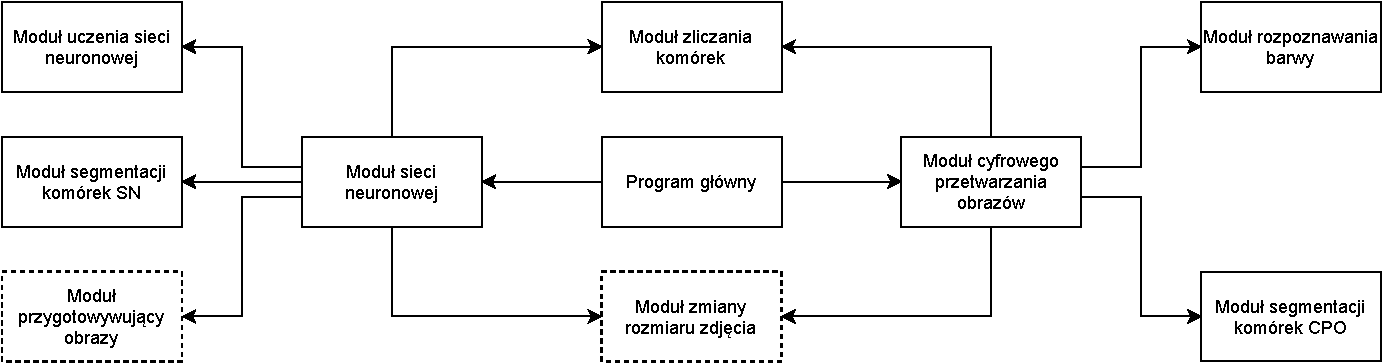
\includegraphics[width=1\textwidth, height=0.2\textheight, trim={0cm 0cm 0cm 0cm}]{diagram.pdf}
    \caption{Diagram modułów}
    \label{fig:diagram}
\end{figure}

\section{Pakiety i moduły}
\subsection{Pakiety}
W celu uporządkowania projektu powstaną cztery pakiety, w których będą przechowywane pliki.
\begin{itemize}
    \item main -- pakiet będzie zawierał program główny,
    \item dip -- pakiet będzie zawierał moduły/pliki związane z cyfrowym przetwarzaniem sygnałów,
    \item nn -- pakiet będzie zawierał moduły/pliki związane z sieciami neuronowymi,
    \item shared -- pakiet będzie zawierał moduły/pliki, które będą wspólne dla~cyfrowego przetwarzania sygnałów i sieci neuronowych.
\end{itemize}
\subsection{Podział modułów}
Moduły możemy podzielić na trzy następujące kategorie -- moduły dla cyfrowego przetwarzania obrazów, moduły dla sieci neuronowych oraz moduły wspólne dla~dwóch różnych podejść. Każdy z modułów będzie osobnym plikiem, który będzie miał określone zadanie do wykonania oraz jedną lub więcej zaimplementowanych funkcji. Każdy moduł będzie zawarty w odpowiednim pakiecie. Poniżej zostanie opisana koncepcja każdego z modułów.
\subsection{Moduły cyfrowego przetwarzania obrazów}
\begin{itemize}
    \item Moduł cyfrowego przetwarzania obrazów
    \newline
    Nazwa modułu: \textit{digital\_image\_processing.py}
    \newline
    Moduł jest odpowiedzialny za uruchamianie innych modułów w obszarze cyfrowego przetwarzania sygnałów.
    \item Moduł rozpoznawania barwy 
    \newline
    Nazwa modułu: \textit{colour\_recognition.py}
    \newline
    Moduł jest odpowiedzialny za poprawne rozpoznanie, czy obraz składa się z pikseli w odcieniach szarości, czy z pikseli kolorowych. 
    \item Moduł segmentacji komórek CPO
    \newline
    Nazwa modułu: \textit{segmentation\_dip.py}
    \newline
    Moduł jest odpowiedzialny za przygotowanie zdjęcia z wysegmentowanymi komórkami gotowymi do zliczenia.
\end{itemize}
\subsection{Moduły sieci neuronowej}
\begin{itemize}
    \item Moduł sieci neuronowej
    \newline
    Nazwa modułu: \textit{neural\_network.py}
    \newline
    Moduł jest odpowiedzialny za uruchamianie innych modułów w obszarze sieci neuronowych.
    \item Moduł uczenia sieci neuronowej
    \newline
    Nazwa modułu: uzależniona od implementacji sieci neuronowej
    \newline
    Moduł ten zostanie dostarczony przez wybraną implementację sieci neuronowej oraz będzie służył do uczenia sieci neuronowej.
    \item Moduł segmentacji komórek SN
    \newline
    Nazwa modułu: uzależniona od implementacji sieci neuronowej
    \newline
    Moduł ten zostanie dostarczony przez wybraną implementację sieci oraz będzie służył do segmentacji komórek na zdjęciach mikroskopowych.
    \item *Moduł przygotowywujący obrazy
    \newline
    Nazwa modułu: \textit{prepare\_images.py}
    \newline
    W przypadku potrzeby powstania tego modułu, będzie on odpowiedzialny za przygtowania danych do uczenia sieci neuronowj, to znaczy dostosowania aktualnych katalogów z obrazami i maskami do wybranej implementacji sieci neuronowej.
\end{itemize}
\subsection{Moduły współdzielone}
\begin{itemize}
    \item Moduł zliczania komórek
    \newline
    Nazwa modułu: \textit{counter.py}
    \newline
    Moduł jest odpowiedzialny za zliczenie wysegmentowanych komórek, zarówno w przypadku cyfrowego przetwarzania obrazów, jak i sztucznych sieci neuronowych. Moduł będzie wykorzystywał biblioteki, takie jak \textit{OpenCV}, czy \textit{scikit-image}.
    \item *Moduł zmiany rozmiaru zdjęć
    \newline
    Nazwa modułu: \textit{change\_images\_size.py}
    \newline
    W przypadku potrzeby powstania tego modułu, będzie on odpowiedzialny za zmianę rozmiaru zdjęć, do takiej przy której będą uzyskiwane najlepsze wyniki. Moduł może zostać wykorzystany w przypadku potrzeby normalizacji rozmiaru zdjęć dla sieci neuronowej.
\end{itemize}


\section{Algorytm}
Algorytmy każdego z dwóch różnych podejść do rozwiązania problemu będą przede wszystkim zaimplementowane w modułach segmentacji komórek CPO i~SN. W przypadku cyfrowego przetwarzania obrazów, dodatkowo możemy włączyć w to zagadnienie moduł rozpoznawania barw. Poniżej zostaną opisane szczegółowo elementy, które będą wykorzystane w algorytmach.
\subsection{Cyfrowe przetwarzanie obrazów}
Realizacja algorytmu za pomocą cyfrowego przetwarzania obrazów obejmować będzie dwa moduły, a dokładnie moduł segmentacji komórek CPO oraz moduł rozpoznawania barw, co jest związane z jakością obrazu. W przypadku obrazów w odcieniach szarości, tło jest jednolite (zazwyczaj czarny kolor), dzięki czemu obraz jest dobrej jakości pomimo rozmycia komórek. W przypadku obrazów kolorowych, tło jest bardzo rozmyte, co może wymagać innej obróbki obrazu w~celu segmentacji komórek. Z tego powodu, na początku zostanie przeprowadzona kwalifikacja obrazu w celu określenia, czy obraz jest w odcieniach szarości, czy jest kolorowy.
\newline \newline
Specyfika projektu nie pozwala na zaprojektowanie algorytmu, ze względu na~fakt, iż będzie on tworzony emiprycznie. Natomiast możemy wyróżnić kilka dużych etapów w algorytmie, które zostaną zrealizowane.
\begin{enumerate}
    \item Usunięcie rozmycia obrazów za pomocą wybranych operacji.
    \item Wykrycie krawędzi za pomocą określonych operacji.
    \item Segmentacja komórek na obrazie.
\end{enumerate}
W celu zrealizowania powyższych kroków zostaną wykorzystane techniki, takie jak:
\begin{itemize}
    \item filtracja -- pozwala na przetwarzanie obrazu w celu zmiany, bądź uwypuklenia jego cech. Dzięki filtracji możemy usunąć szumy róznego rodzaju oraz poprawić jakość obrazu.
    \item segmentacja -- pozwala na wyodrębnienie części obrazu, która reprezentuje pewien obiekt poprzez zmianę wartości pikseli na taką samą w ramach określonego obiektu. Najprostszym przykładem segmentacji obrazu w odcieniach szarości może być binaryzacja.
    \item binaryzacja -- pozwala na przekształcenie obrazu w jednowymiarowy obraz, gdzie każdy punkt może przyjąć kolor biały bądź czarny. Operacja ta może być przydatna podczas segmentacji. Wykorzystana może zostać metoda Otsu.
    \item morfologia matematyczna -- dziedzina ta pozwala wykonywać operacje na~obrazach z wykorzystaniem masek, które mają wpływ na~ostateczną wartość danego punktu. Może być wykorzsytana do wykrywania krawędzi za~pomocą gradientu morfologicznego.
\end{itemize}
Projekt algorytmu w znacznej części zostanie oparty o następujące biblioteki:
\begin{itemize}
    \item numpy -- biblioteka wspomagająca obsługę wektorów oraz macierzy,
    \item matplotlib -- biblioteka do tworzenia wykresów,
    \item skimage (scikit-image) -- biblioteka dedykowana do przetwarzania obrazów,
    \item cv2 (OpenCV) -- biblioteka wspierająca przetwarzanie obrazów.
\end{itemize}

\subsection{Sieć neuronowa}
Sieci neuronowe są bardzo obszernym tematem. Cechują się one różnorodnością pod względem nie tylko rodzaju sieci neuronowej, ale także implementacji. Określona sieć neuronowa może zostać zaimplementowana w różnych językach, bazując na różnorodnych bibliotekach. W przypadku języka \textit{Python}, do najpopularniejszych możemy zaliczyć biblioteki, takie jak \textit{TensorFlow}, \textit{Keras} czy \textit{PyTorch}.
\newline \newline
Na początku należy określić rodzaj sieci neuronowej, jaka zostanie wykorzystana w projekcie w celu segmentacji komórek na zdjęciach mikroskopowych. Przypuszczalnie najlepszym rozwiązaniem będzie wykorzystanie konwolucyjnych sieci neuronowych. Sieci te są wzbogacone o dodatkowe możliwości ekstrakcji, bądź uwypuklenia cech na obrazach. Jest to efekt określonych filtracji sygnałów zastosowanych na obrazach. Możemy osiągnąć taki efekt, ze względu na fakt, iż~cyfrowe przetwarzanie obrazów jest częścią cyfrowego przetwarzania sygnałów, natomiast przetwarzane sygnały możemy traktować jako obraz.
\newline
Kolejnym etapem jest wybór konkretnej konwolucyjnej sieci neuronowej. W~tym celu zostaną zaproponowane dwa rozwiązania, a ostateczna decyzja zostanie podjęta na podstawie wstępnego zapoznania się z określonymi sieciami neuronowymi. Poniżej zostaną krótko opisane wybrane wstępnie sieci neuronowe.
\begin{itemize}
    \item U-Net -- konwolucyjna sieć neuronowa, zaprojektowana do segmentacji obrazów biomedycznych na Uniwersytecie we Freiburgu.
    \item Mask R-CNN (Mask Region Based Convolutional Neural Networks) -- konwolucyjna sieć neuronowa pochodząca z rodziny sieci neuronowych R-CNN, która przestała koncentrować się na wykrywaniu obiektów, na rzecz ich segmentacji. Jest ona rozwijana przez firmę \textit{Facebook}.
\end{itemize}
Ostatnią rzeczą jaką należy okrelić w przypadku sieci neuronowej, to jej implementacja. Niezależnie od wyboru sieci neuronowj (pierwsza, bądź druga opisana sieć neuronowa) zostanie wybrana implementacja z użyciem biblioteki \textit{PyTorch}. 
\section{Testowanie}
\subsection{Proces testowania}
Proces testowania jest całkowicie uzależniony od podejścia do rozwiązania problemu. Dlatego poniżej zostaną zaprezentowane dwie różne propozycje przeprowadzenia procesu testowania.
\subsection{Cyfrowe przetwarzanie obrazów}
W przypadku cyfrowego przetwarzania obrazów, możemy wykorzystać fakt, iż w zbiorze jest zestaw \textit{stage1\_train} przeznaczony do trenowania sieci neuronowej. Zestaw ten oprócz obrazów z komórkami zawiera zestaw masek dla każdego z~obrazów, co pozwala nam zidentyfikować liczbę komórek na zdjęciu mikroskopowym. Rodzaj tej metody pozwala nam wykorzystać uprzednio wymieniony fakt, ze względu na to, że nie wymaga ona procesu uczenia, a zatem oryginalne zdjęcia oraz maski nie zostaną wcześniej przez nią wykorzystane.
\newline \newline
Niewykluczone, że w celu zautomatyzowania tego zadania powstanie skrypt w~języku \textit{Python} o nazwie \textit{count\_accuracy.py}, który będzie w stanie wyznaczyć dokładność algorytmu. Skrypt ten będzie wyznaczał dokładność dla jednego obrazu, jako stosunek komórek znalezionych przez program do liczby masek dla danego obrazu. Następnie wynik zostanie uśredniony dla określonej próbki obrazów.
\subsection{Sieć neuronowa}
 W przypadku sieci neuronowej możemy zastosować dwa podejścia. Pierwsze z~nich wymaga zidentyfikowania oraz manualnego zliczenia komórek na obrazach ze zbioru \textit{stage1\_test} oraz porównania ich z otrzymanymi wynikami.
 \newline \newline
 Dodatkowo można wyznaczyć część zbioru, która będzia określona jako podzbiór walidacyjny. Bardzo często takie rozwiązanie jest stosowane, natomiast jest ono uzależnione od wybranej implementacji sieci neuronowej. W takiej sytuacji, użytkownik określa jaki procent obrazów posłuży jako zbiór walidacyjny, a następnie sieć neuronowa wyznacza sama dokładność na podstawie wysegmentowanych elementów.
\label{end}
\end{document}